% !TeX spellcheck = en_GB
%****************************************************
%	CHAPTER 2 - SLAM overview
%****************************************************
\chapter{SLAM overview}
\label{ch:ch2}
%====================================================
In this chapter, a review of SLAM fundamentals is presented. Background concepts are discussed to establish a framework for the map merging problem presented in later chapters, and basic concepts of autonomous mobile robot systems are introduced as a basis for the SLAM framework.
%====================================================
\section{Autonomous robot system overview}
\label{section:ARSO}
%----------------------------------------------------
Imagine a mobile robot has been given a mission to explore an unknown environment. To achieve this mission, the robot first gathers data from the unfamiliar environment (\textbf{perception}), then maps and localises itself within the environment (\textbf{SLAM}), followed by developing a plan on how to move through the world based on the goal of the mission (\textbf{navigation} and \textbf{path planning}). Finally, it initiates the robot's controlled motion along the decided path (\textbf{motion control}). Each module in the system is dependent on the quality of outputs from the previous modules. For example, to perform path planning successfully, a high-quality map is needed from the SLAM block, which requires that the data collected from the environment by the perception block is of a suitable format, scale and resolution to generate a map and localise the robot within it. In the sections that follow, the perception and SLAM blocks are explored in detail and, while an in-depth explanation of path planning and motion control is omitted, the output of the SLAM sub-system will be discussed concerning required input to the path planning module.

%....................................................
\begin{figure}[H]
%----------------------------------------------------
	\centering
	\includegraphics[width=1\linewidth]{"figs/autonomus_overview"}
%----------------------------------------------------	
	\caption[Autonomous robot system overview]{A high-level overview of a typical autonomous mobile robot system. Illustrating the interactions between the real-world environment, its perceptions system, the robots internal model of the world, its planning unit and finally its motion control centre. Adapted from \cite{Siegwart2004}.}
%----------------------------------------------------	
	\label{fig:autoover}
%----------------------------------------------------	
\end{figure}
%....................................................

Figure \ref{fig:autoover} is an illustration of an Autonomous Robot System (ARS) where different interdependent modules are displayed, each module both receives and shares information with other modules in the system \cite{Siegwart2004}. 

%====================================================
\section{Perception system}
%----------------------------------------------------
For an ARS to interact with the real world, it needs to acquire information about the environment as it moves through it. This process is referred to as perception and involves taking measurements using multiple sensors followed by extracting useful information from these measurements. There are various sensors one can choose from when designing an autonomous robot system and depend on the type of robot platform and the environmental context in which it will operate. For example, a terrestrial robot might use GNSS positioning systems, inertial measurement units (IMU), Light Detection and Ranging (LIDAR), RADAR, and cameras to take both the robot's measurements internal state and external environmental variables. In contrast, underwater robots might use a combination of SONAR and inertial sensors. A robot's perception system can sense both internal properties of the robot and external properties of the environment \cite{Siciliano2008b}. These sensors can be primarily classified as exteroceptive/proprioceptive and active/passive. 

\textbf{Exteroceptive} sensors acquire information about the external environment. For example, distance and angle measurements from the robot to objects in the environment, environmental light intensity or acoustic amplitude. Therefore, exteroceptive sensors are used by the robot to extract information about the state of the environment. \textbf{Proprioceptive} sensors measure internal parameters of the robot; for example, wheel rotations, motor speed, angular velocity, linear acceleration and battery current/voltage.

Furthermore, sensors can also be distinguished by whether they are active or passive, i.e. whether they emit energy into the environment or not. \textbf{Passive} sensors measure ambient energy from the environment; for example, temperature probes, microphones and cameras. \textbf{Active} sensors, such as LIDAR, stimulate the environment by emitting energy into it and then measure the reaction from the environment.

Most mobile robots use some form of \textbf{range sensor} to measure their relative position to objects in the environment. These sensors include ultrasonic, infrared (IR), stereo cameras, RADAR and LIDAR devices. A range sensor gives the distance to the nearest object in a given direction. Range sensors, typically, form the basis of methods for detecting obstacles in the environment and as inputs to map generation and localisation. Range sensors also play a role in correcting odometry errors where they are present.

\textbf{Odometry} refers to the use of the motion of actuators such as wheels and treads, to estimate the overall motion of a robot. This estimation is based on developing a mathematical model of how actuator motion induces motion on the robot itself. This motion mapping is integrated over time to develop a model of the robot's pose as a function. This process of estimating the pose is known as \textbf{dead reckoning} \cite{Siciliano2008b}. Even though odometry sensors provide information about robot motion, the information accumulates errors over time, which are not corrected by the sensors themselves. In many cases, LIDAR and GPS are used used to complement odometric information \cite{Grisetti2007}.

The perception system provides input information to the localisation and map building (SLAM) modules, which need to process the data further to extract a map model of the environment and localise the robot within it. The following section discusses the SLAM module in more detail.

%For example in \cite{Grisetti2007} the probability distribution of \(P(z|x)\) is more peaked than \(P(x_t|x_{t-1}|u_t)\), this means that probability of the LIDAR measurement \(z\) given the pose\(x_t\) of the robot  at time \(t\) is more certain than the probability of pose of the robot \(x_t\) given previous pose \(x_{t-1}\) and odometric reading \(u\).
%
%==================================================== 
\section{SLAM process}
%----------------------------------------------------
%Leading up to the localisation and map building block(see Figure \ref{fig:autoover}), Simultaneous Localisation and Mapping(SLAM) is introduced. % 

SLAM builds a new map of an unknown environment or updating an existing map, while simultaneously localising the robot within the map \cite{Bailey2006b}. There are many techniques used to handle errors generated by the system. These techniques include feature detection between steps \cite{Kim2007a}, data association \cite{Nieto2003} or loop closure detection\cite{Labbe2014}. SLAM is mainly solved using a probabilistic approach, as the robot's perception system has an uncertainty associated with measurements and inherent sensor noise.

%Bayes rule can be used to deal with the imperfections of the motion model and sensor inputs.
%....................................................
\begin{figure}[H]
%----------------------------------------------------
	\centering
	\includegraphics[width=0.7\linewidth]{"figs/slam"}
	
%----------------------------------------------------	
	\caption[Graphical representation of SLAM process]{Graphical representation of the SLAM  process. As a robot (\robot) moves through (\redline) an environment, which contains a series of discrete landmarks (\landmark), it needs to simultaneously estimate the locations of the landmarks (\landmarkest) and itself (\robotest) relative to the mapped landmarks.  The locations of both the robot ($\mathbf{x}_{k}$) at time $k$ and the $i^{th}$ landmark ($\mathbf{m}_{i}$) are estimated from observations (\bluearrow, $\mathbf{z}_{k}$) taken by the robot's perception system and models of the robot's motion overtime after a control input ($\mathbf{u}_{k}$) has been applied to the robot at time $k-1$. Additionally, it uses this information to build up a history of its trajectory through the environment (\orangedashed, $\mathbf{X}_{0:k}$). Modified from \cite{Bailey2006}.}
%----------------------------------------------------	
	\label{fig:slam-problem}
%----------------------------------------------------	
\end{figure}
%....................................................

The SLAM problem can be formulated as follows\footnote{\textbf{Note:} The notation used in formulating the SLAM problem is largely based on \cite{Bailey2006b}.} : Continuing with the scenario described in Section\ref{section:ARSO}, a mobile robot enters an environment, which contains a number of discrete landmarks, whose true locations are assumed to be time-invariant. As it moves through the environment it needs to simultaneously produce a map ($m$ of all the estimated landmark positions in the environment ($\mathbf{m}=\{\mathbf{m}_1, \mathbf{m}_2,\dots{}, \mathbf{m}_n\}$), where $\mathbf{m}_{i}$ is a vector representing the estimated location of the $i^{th}$ landmark in a set of $n$ observed landmarks, and estimate the robot's trajectory ($\mathbf{X}_{0:k}$), where ($\mathbf{X}_{0:k}=\{\mathbf{x}_{0}, \mathbf{x}_{1}, \dots{}, \mathbf{x}_{k}\}$) is a set of all estimated robot poses within the environment over time, starting from an initial state $\mathbf{x}_{0}$. $\mathbf{x}_{k}$ is a state vector describing the global location and orientation of the vehicle, at time $k$, where  $k \in{} \{0,1,\dots{},k\}$. 

For the robot to move from one location ($\mathbf{x}_{k-1}$) to the next  ($\mathbf{x}_{k}$),  a control input $\mathbf{u}_{k}$, is applied to the robot at time $k-1$. $\mathbf{U}_{0:k}=\{\mathbf{u}_1, \mathbf{u}_2,\dots{}, \mathbf{u}_k\}$ is a set of all the control inputs applied to the robot to move it from its initial state $\mathbf{x}_{0}$ to its current state $\mathbf{x}_{k}$. At each sample in time, $k$, the robot takes measurements $\mathbf{z}_{i,k}$ of the relative position and pose between its true location and the $i^{th}$ landmark. $\mathbf{z}_{k}$ represents the observations to all detectable landmarks at time $k$ and $\mathbf{Z}_{0:k}=\{\mathbf{z}_0, \mathbf{z}_1,\dots{}, \mathbf{z}_k\}$ is the history of the relative position measurements to all observed landmarks for from the initial to the current location. See Figure \ref{fig:slam-problem} for a graphical representation of the process.

%The SLAM problem was first solved in the 1980s by Smith and Cheeseman \cite{}, based on state estimation techniques \cite{}. The estimation problem was solved using the \textit{recursive Bayesian filter}. In the approach, the Bayes filter performs an iterative prediction\xrightarrow{} correction cycle to integrate new sensor data, while marginalising out the previous robot pose $\mathbf{x}_{k-1}$. The approach models the SLAM problem as a first-order discrete-time Markov chain, where the future is assumed to be independent of the past, given the present state. The Bayes filter below uses an odometry-based model, while Thrun provides a more general Bayes filter in \cite{}.

The uncertainty in robotics can be represented using the calculus of probability theory, which instead of relying on a single \textit{``guess''}, the probabilistic algorithms represent information by a probability distributions over a whole space of guesses. The probabilistic form of SLAM uses Bayes Theorem to estimate the \textbf{joint posterior} probability distribution $(bel(\mathbf{x}_{k},\mathbf{m}))$, for both the current robot state ($\mathbf{x}_{k}$) and map ($\mathbf{m}$) at time $k$ given a history of all observations $\mathbf{Z}_{0:k}$  and control $\mathbf{U}_{0:k}$ inputs to the platform from its initial state $\mathbf{x}_{0}$ to its current state $\mathbf{x}_{k}$, 
%....................................................
\begin{equation}
%----------------------------------------------------
    bel(\mathbf{x}_{k},\mathbf{m}) = P(\mathbf{x}_{k},\mathbf{m}|\mathbf{Z}_{0:k},\mathbf{U}_{0:k},\mathbf{x}_{0}).
%----------------------------------------------------
\label{eq:slamproblem}
%---------------------------------------------------- 
\end{equation}
%....................................................

The SLAM algorithm is implemented in two recursive steps, time-update $\rightarrow$ measurement-update to integrate new sensor data while marginalising out the previous robot pose $\mathbf{x}_{k-1}$. The prediction step incorporated the control input ($\mathbf{u}_k$), and the measurement-update incorporates the measurement ($\mathbf{z}_k$) into the posterior, hence their respective naming. The approach models the SLAM problem by assuming that the dynamics are Markov, where the future is assumed to be independent of the past, given the present state. The Bayes filter below uses an odometry-based model, while Prof. Thrun provides a more general Bayes filter in \cite{Thrun2006}. The steps are in the following form:

%is solved recursively at each time step, using the previously estimated joint posterior probability $P(\mathbf{x}_{k-1},\mathbf{m}|\mathbf{Z}_{0:k-1},\mathbf{U}_{0:k-1})$ and a robot motion model $P(\mathbf{x}_{k}|\mathbf{x}_{k-1},\mathbf{u}_{k})$ and an observation model $P(\mathbf{z}_{k}|\mathbf{x}_{k},\mathbf{m})$, which describe the effects of the control input and observation respectively.

\textbf{Time-Update:} The current robot state is predicted using the prior belief $bel(\mathbf{x}_{k-1}) = P(\mathbf{x}_{k-1},\mathbf{m}|\mathbf{Z}_{0:k-1}, \mathbf{U}_{0:k-1}, \mathbf{x}_{0})$ and the robot’s motion model (with associated assumptions such as constant velocities). Using the law of total probabilities, the prior belief $bel(\mathbf{x}_{k-1})$ is marginalised out to form the prediction $\bar{bel}(\mathbf{x}_k)$:
%....................................................
\begin{equation}
%----------------------------------------------------
\begin{split}
%----------------------------------------------------
%\text{\textbf{Time-Update}} \\
    \bar{bel}(\mathbf{x}_k, \mathbf{m}) = \underbrace{P(\mathbf{x}_k,\mathbf{m}|\mathbf{Z}_{0:k-1}, \mathbf{U}_{0:k}, \mathbf{x}_0)}_{\text{prediction}} = \int  \underbrace{P(\mathbf{x}_k|\mathbf{x}_{k-1},\mathbf{u}_k)}_{\text{motion model}} \times \underbrace{P(\mathbf{x}_{k-1},\mathbf{m}|\mathbf{Z}_{0:k-1}, \mathbf{U}_{0:k-1}, \mathbf{x}_0)}_{\text{prior belief}} d_{\mathbf{x}_{k-1}}
%----------------------------------------------------    
\end{split}
%----------------------------------------------------
\label{eq:timeup}
%----------------------------------------------------
\end{equation}
%....................................................

Here, the motion model describes the probability of robot's pose, $\mathbf{x}_k$, given the preceding pose, $\mathbf{x}_{k-1}$, and the applied control input, $\mathbf{u}_k$. The motion model is assumed to be a Markov process independent of both observation, $\mathbf{z}_k$, and map, $\mathbf{m}$.

\textbf{Measurement-Update:} The posterior belief ($bel(\mathbf{x}_k)$) is then formed using Bayes rule to form:

%....................................................
\begin{equation}
%----------------------------------------------------
\begin{split}
%----------------------------------------------------
%\text{\textbf{Measurement-Update}} \\
%----------------------------------------------------
bel(\mathbf{x}_k, \mathbf{m}) = \underbrace{P(\mathbf{x}_k,\mathbf{m}|\mathbf{Z}_{0:k}, \mathbf{U}_{0:k}, \mathbf{x}_0)}_{\text{posterior}} &= \frac{\overbrace{P(\mathbf{z}_k|\mathbf{x}_{k},\mathbf{m})}^{\text{observation model}} \overbrace{P(\mathbf{x}_k,\mathbf{m}|\mathbf{Z}_{0:k-1}, \mathbf{U}_{0:k}, \mathbf{x}_0)}^{\text{prediction}}}{P(\mathbf{z}_k|\mathbf{Z}_{0:k-1},\mathbf{U}_{0:k})} \\
%----------------------------------------------------
&= \eta \overbrace{P(\mathbf{z}_k|\mathbf{x}_{k},\mathbf{m})}^{\text{observation model}} \overbrace{P(\mathbf{x}_k,\mathbf{m}|\mathbf{Z}_{0:k-1}, \mathbf{U}_{0:k}, \mathbf{x}_0)}^{\text{prediction}}
%----------------------------------------------------
\end{split}
%----------------------------------------------------
\label{eq:measureup}
%----------------------------------------------------
\end{equation}
%....................................................

Here, the observation model $P(\mathbf{z}_k|\mathbf{x}_{k},\mathbf{m})$ describes the probability of an observation, $\mathbf{z}_k$, when a robot's pose,$\mathbf{x}_k$, and map/landmark locations, $\mathbf{m}$, are known. Assuming that a robot's pose, $\mathbf{x}_k$, and map/landmark locations, $\mathbf{m}$, are defined, observations are conditionally independent given the map and current robot pose. The term $P(\mathbf{z}_k|\mathbf{Z}_{0:k-1},\mathbf{U}_{0:k})$ does not depend on $\mathbf{x}$ and in practice this term is not calculated; rather the posterior distribution is normalised to one \cite{Thrun2006}. The normalisation term $\eta$, is therefore, given by $\eta = 1/P(\mathbf{z}_k|\mathbf{Z}_{0:k-1},\mathbf{U}_{0:k})$.

Therefore in a Bayes filter the joint posterior for $P(\mathbf{x}_k,\mathbf{m}|\mathbf{Z}_{0:k}, \mathbf{U}_{0:k}, \mathbf{x}_0)$ can be calculated recursively using equations \ref{eq:timeup} and \ref{eq:measureup}, given all observations $\mathbf{Z}_{0:k}$ and all control inputs $\mathbf{U}_{0:k}$ up to and including the current time $k$. 

The time-update and measurement-update can then be represented as an algorithm. Algorithm \ref{alg:bayes_filter}, describes the time-update step $\bar{bel}(\mathbf{x}_k)$ which predicts the state of the mobile robot at time $k$ based on previous sate posterior without incorporating the measurement at time $k$, and the measurement-update step $bel(\mathbf{x}_k)$ which incorporates the measurement to improve the posterior belief distribution.

%....................................................
\begin{algorithm}[H]
%----------------------------------------------------
	\SetAlgoLined
	\KwData{$bel(x_{k-1}), u_k, z_k$}
	
	\For{all $x_k$}{
		$\bar{bel}(x_k) = \int p(x_k|u_k,z_k)  bel(x_{k-1}) dx_{k-1} $\;
		$bel(x_k) = \eta p(z_k|x_k) \bar{bel}(x_k) $\;
		
	}
	\Return $bel(x_k)$
%----------------------------------------------------	
	\caption[Bayes Filter]{The algorithm calculates the belief distribution $bel$ from measurements $\mathbf{z}_k$ and control inputs $\mathbf{u}_k$. The belief $bel(\mathbf{x}_k)$ is calculated from $bel(\mathbf{x}_{k-1}), \mathbf{u}_k, \mathbf{z}_k$, where the $\mathbf{z}_k$ and $\mathbf{u}_k$ are the most recent measurements and input control \cite{Thrun2006}, where $bel(x_k) = P(x_k,m|Z_{0:k}, U_{0:k},x_0)$. This is well illustrated in \ref{fig:slam-problem}, where the SLAM problem is shown.}\label{alg:bayes_filter}
%----------------------------------------------------
\end{algorithm}
%....................................................

With SLAM's foundations established, the following section will expand on some of the most commonly used approaches.

%====================================================
\section{SLAM approaches}
%----------------------------------------------------
Expanding on the above-mentioned probabilistic approach to SLAM, several methods can solve the SLAM problem, which involves finding an appropriate representation for both the observation and motion models, that allow efficient computation of the prior (\ref{eq:timeup}) and posterior (\ref{eq:measureup}) distributions. The three most commonly used SLAM solutions are EKF-SLAM, Fast-SLAM and Graph-SLAM. However, new methods such as Hector-SLAM are also useful. The following section explored the solutions mentioned above, even though there are many alternative approaches \cite{Seminar2016}.

%----------------------------------------------------
\subsection{EKF-SLAM}
\label{subsec:ekf-slam}
%----------------------------------------------------
The Extended Kalman Filter (EKF) is the most common representation as it is one of SLAM's earliest implementation. The basic Kalman Filter implementation only deals with linear systems with Gaussian noise, and the EKF implementation extends to nonlinear systems \cite{Li2012}. The EKF replaces the Kalman Filter motion model with a nonlinear model, as a linear system is rarely observed in the real-world. 

The EKF approach is a state-space model, with additive Gaussian noise. The EKF model was first proposed using a single state vector to estimate the mobile robot's locations and features in an environment, and these estimations included an associated error covariance matrix that represents the uncertainty of results \cite{Chen2013}. During exploration, the state vector and covariance matrix are updated using the environment measurements and an EKF is introduced \cite{Bailey2006b}. The covariance matrix grows quadratically as new features are observed, and thus new states are added.

In the EKF, the nonlinear model is linearised using a Taylor expansion around the current state estimate \cite{Kurt-Yavuz2012}. Where, the current state is represent by a mean state vector $\mathbf{\mu}_k = [\mathbf{x}_k, \mathbf{m}_1, \mathbf{m}_2, \dots{}, \mathbf{m}_n]^T $ as well as a covariance matrix $\mathbf{\Sigma}_k$ which signifies the co-variance between the state variables also a measure of confidence at time $k$. As with the general Bayes filter, the EKF approach iterates between the time-update $\rightarrow$ measurement-update cycle. A brief overview is given mathematically in the rest of this section. In chapter 10 of \cite{Thrun2006}, Thrun et al. present an in-depth EKF based SLAM tutorial.

\textbf{Time-Update:} In this stage the filter computes the co-variance matrix $\bar{\mathbf{\Sigma}}_k$ and predicted the state vector $\bar{\mathbf{\mu}}_k$ and time $k$:

%....................................................
\begin{equation}
%----------------------------------------------------
\begin{split}
%----------------------------------------------------
    \mathbf{\bar{\mu_k}} &= g(\mathbf{u}_k, \mathbf{\mu}_{k-1})\\
	\mathbf{\bar{\Sigma_k}} &= \mathbf{G}_k \mathbf{\Sigma}_{k-1} \mathbf{G}^{T}_{k} + \mathbf{R}_k,
%----------------------------------------------------	
\end{split}
%----------------------------------------------------
	\label{eq:ekf:time}
\end{equation}
%....................................................

Here, $g$ is the motion model of the robot updated using given odometry. The covariance matrix $\mathbf{\bar{\Sigma_k}}$ is updated by the motion model's Jacobian $\mathbf{G}_k = \frac{\delta g }{ \delta \mathbf{\mu}_{k-1}}$ and the process noise $\mathbf{R}_k$. The process noise results from the motion model, which is assumed to be additive and is typically the same as the odometry noise.


\textbf{Measurement-Update:} In this stage, updated measurement of state vector ${\mathbf{\mu}_k}$ and it is associated ${\bar{\Sigma_k}}$ are computed, by first computing the Kalman gain $\mathbf{K}_k$. The Kalman gain $\mathbf{K}_k$ is the relative weight given to the measurements and current state estimate given by Equation \ref{eq:ekf:gain}.


%....................................................
\begin{equation}
%----------------------------------------------------
	\mathbf{K_k} = \bar{\mathbf{\Sigma}}_k \mathbf{H}_{k}^T(\mathbf{H}_k\bar{\mathbf{\Sigma}}_{k-1}\mathbf{H}_{k}^T+\mathbf{Q}_k)^{-1}
%----------------------------------------------------	
	\label{eq:ekf:gain}
%----------------------------------------------------
\end{equation}
%....................................................

Here, the sensor model's Jacobians $\mathbf{H}_k = \frac{\delta h}{\delta \bar{\mathbf{\mu}_k}}$ apply a linearisation and the sensor model noise is incorporated by the co-variance $\mathbf{Q}_k$. This gain can be tuned to achieve a particular performance; with a higher gain placing more weight on current measurements and lower gain, placing more weight on the prediction \cite{Thrun2006}. 

The Kalman gain is then used to compute the posterior estimate state vector, $ \mathbf{\mu}_k$,and its associated covariance matrix $\mathbf{\Sigma}_k$.

%....................................................
\begin{equation}
%----------------------------------------------------
\begin{split}
%----------------------------------------------------
    \mathbf{\mu}_k &= \bar{\mathbf{\mu}_k} + \mathbf{K}_k(\mathbf{z}_k-h(\bar{\mathbf{\mu}_k}))\\
	\mathbf{\Sigma}_k &= (\mathbf{I} -\mathbf{K}_k \mathbf{H}_k)\bar{\mathbf{\Sigma}_k}
%----------------------------------------------------	
\end{split}
%----------------------------------------------------
	\label{eq:ekf:measure}
%----------------------------------------------------	
\end{equation}
%....................................................

Here, $h$ is the sensor model and $\mathbf{z}_k$ is the sensor measurements. The posterior $\mathbf{\mu}_k$ contains updated estimates for the state vector, which includes both the robot’s pose $\mathbf{x}_k$ and $\mathbf{m}=\{\mathbf{m}_1, \mathbf{m}_2,\dots{}, \mathbf{m}_n\}$), where $\mathbf{m}_{i}$ landmarks


Algorithm \ref{alg:ekf-algorithm} shows the summarised Extended Kalman Filter algorithm used to compute the Gaussian posterior in \ref{eq:ekf:time}, where $\mathbf{\mu}_k = [\mathbf{x}_k, \mathbf{m}_1, \mathbf{m}_2, \dots{}, \mathbf{m}_n]^T $ is a mean vector and $\mathbf{\Sigma}_k$ is a co-variance matrix at time $k$. 


%....................................................
\begin{algorithm}[H]
%----------------------------------------------------
	\SetAlgoLined
	\KwData{\(\mu_{k-1}, \Sigma_{k-1}, u_k, z_k \)}
	    \(\bar{\mu_k} = g(u_k, \mu_{k-1})\)\;
	    \(\bar{\Sigma_k} = G_k \Sigma_{k-1} G^{T}_{k} + R_k\)\;
    	\(K_k = \bar{\Sigma_k} H^T_k(H_k\bar{\Sigma_k}H^T_k + Q_k)^{-1}\)\;
	    \(\mu_k = \bar{\mu} + K_k(z_k-h(\bar{\mu_k}))\)\;
    	\(\Sigma_k = (I -K_k H_k)\bar{\Sigma_k}\)\;
	\Return \(\mu, \Sigma\)
%----------------------------------------------------	
	\caption[Extended Kalman Filter Algorithm]{Extended Kalman Filter Algorithm\cite{Thrun2006}, where $\mathbf{\mu}_k = [\mathbf{x}_k, \mathbf{m}_1, \mathbf{m}_2, \dots{}, \mathbf{m}_n]^T $ is a mean vector, $\mathbf{\Sigma}_k$ is a co-variance matrix at time $k$}\label{alg:ekf-algorithm}
%----------------------------------------------------	
\end{algorithm}
%....................................................

EKF-SLAM employs linearised models of nonlinear motion and observation models, where errors are introduced by linearisation. At each time step, $k$, as the robot moves in the environment, its current pose uncertainty increases, the uncertainty is reduced by recurringly observing landmarks. This process in EKF-SLAM aims to marginalise out the previous estimate $\mathbf{\mu}_{k-1}$, to only incorporate the most recent linearisation errors into the current state $\mathbf{\mu}_{k}$. This process helps limit pose errors that accumulate due to linearisation and odometry errors. Thus, an EKF will always underestimate uncertainties and eventually become inconsistent \cite{CASTELLANOS2004716, 4058955}. An alternative formulation aimed to improve the inconsistencies is proposed in Castellanos et al.; Where, a robot-centred coordinate system is employed to delay the inherent inconsistency \cite{CASTELLANOS2004716, Castellanos2007}, which is adopted in \cite{5509248, Civera2010} too.

The EKF-SLAM solution is fragile to incorrect data association of landmark observations, given that the pose representation is uni-modal with no opportunity to track alternative hypotheses. This incorrect data association causes a problem referred to as loop closure. The loop closure problem occurs when a robot revisits a previously visited location after a lengthy expedition \cite{Balcilar2016}; therefore, the problem is compounded in environments where landmarks look different when observed from a different viewpoint \cite{976019}. 

At each time step, $k$, the measurement-update step needs to update all landmarks and the joint covariance matrix, every time an observation, $\mathbf{z}_k$ is made. Inherently, this scales EKF-SLAM with $\mathcal{O}(M^2)$, where M is the number of landmarks in the map $\mathbf{m}$. This scaling limitation of EKF-SLAM curbs the online execution to several hundred landmarks \cite{4631503}. 

Even though implementations using Field Programmable Gate Arrays (FPGAs) have been demonstrated with 1800 features, \cite{4380720}; solutions such as this scale with silicon size, which is ultimately still limited. Other approaches to scale the EKF-SLAM solution to larger map size, propose fragmenting maps into smaller ``sub-maps''. The sub-mapping technique aims to maintain online performance by restricting the map updates to the landmarks around the robot, such as in \cite{Leonard2000, 973391, 938382, VIDALCALLEJA2011654, Quraishi2016}. However, these methods inherently scale with $\mathcal{O}(M^2)$ on global state and covariance updates.

The method, FastSLAM described in the section to follow attempts to improve the computational, data association and convergence limitations of EKF-SLAM. It was the first model to consider nonlinear models and multi-modal distributions to solve the SLAM problem, with the further advantage of better robustness to loop-closure \cite{Montemerlo2002}. 

%----------------------------------------------------
\subsection{FastSLAM}
%----------------------------------------------------
Montemerlo et al. first introduced FastSLAM in \cite{ Montemerlo2002}, while previous efforts were placed on EKF-SLAM. FastSLAM is a recursive sampling or particle filter, representing the robot pose as a non-Gaussian distribution, unlike the EKF, which represents distributions with a multivariate Gaussian. FastSLAM utilises Rao-Blackwellized Particle Filter, which exploits the conditional independence between landmarks in the fundamental SLAM problem \ref{eq:slamproblem}. Therefore, Rao-Blackwellisation factorises the SLAM problem by separating them into the robot's complete trajectory, $\mathbf{X}_{0:k}$, and map, $\mathbf{m}$, components:

%....................................................
\begin{equation}
%----------------------------------------------------
    \underbrace{P(\mathbf{X}_{0:k}, \mathbf{m}|\mathbf{Z}_{0:k}, \mathbf{U}_{0:k}, \mathbf{x}_0)}_{posterior} = \underbrace{P(\mathbf{m}|\mathbf{X}_{0:k},\mathbf{Z}_{0:k})}_{map}\underbrace{P(\mathbf{X}_{0:k}|\mathbf{Z}_{0:k}, \mathbf{U}_{0:k}, \mathbf{x}_0)}_{trajectory}
%----------------------------------------------------    
\end{equation}
%....................................................

Furthermore, in FastSLAM, the mapping problem is factorised into a separate problem, one for each feature. The features are estimated by two-dimensional EKFs, one for each feature:

%....................................................
\begin{equation}
%----------------------------------------------------
    P(\mathbf{m}|\mathbf{X}_{0:k}^{[q]},\mathbf{Z}_{0:k}) = \prod_{n}^{\mathbf{N}} P(\mathbf{m}_n|\mathbf{X}_{0:k}^{[q]}, \mathbf{Z}_{0:k}).
%----------------------------------------------------    
\end{equation}
%....................................................
This approach is different from the EKF SLAM discussed in the previous Section\ref{subsec:ekf-slam}, where a single Gaussian is used to estimate all features in the map.

FastSLAM maintain $Q$ particles, at some point in time, $k$, where $q$ $(1 \leq q \leq Q)$ particles of:

%....................................................
\begin{equation}
%----------------------------------------------------
\mathbf{X}_{0:k}^{[q]}, \mathbf{\mu}_{k,1}^{[q]}, \dots, \mathbf{\mu}_{k,N}^{[q]}, \mathbf{\Sigma}_{k,1}^{[q]},\dots, \mathbf{\Sigma}_{k,N}^{[q]}
%----------------------------------------------------    
\end{equation}
%....................................................

Here, $[q]$ is the index of the particles. Each particle contains a sample path, $\mathbf{X}_{0:k}^{[q]}$; and a set of \textit{N} two-dimensional Gaussians with means, $\mathbf{\mu}_{k,n}^{[q]}$ and variance, $\mathbf{\Sigma}_{k,n}^{[q]}$ one for each landmark, where $n$ $(1 \leq n \leq N)$ is the index of the landmark. Therefore, $Q$ particles contain $Q$ paths and $QN$ Gaussians that describe landmarks in the environment.

FastSLAM is initialised by setting each particle's robot location to its known starting coordinates and zero the map. Particles are updated in two steps:
\begin{itemize}
    \item \textbf{Time-update}, which is when a new odometry reading $\mathbf{u}_k$ at time $k$ is received, where a new location variable is stochastically generated for each particle. The distribution for generating these particle locations is based on the motion model $\mathbf{x}_k^{[q]} \approx P(\mathbf{x}_k | \mathbf{x}_{k-1}^{[q]}, \mathbf{u}_k)$, where $\mathbf{x}_{k-1}^{[q]}$ is the previous location of particle $M$. 
    \item \textbf{Measurement-Update}, which is when a new measurement $\mathbf{z}_k$ at time $k$ is received. Where, firstly FastSLAM computes the probability of the measurement $\mathbf{z}_k$, defined by 
    %....................................................
    \begin{equation}
    %----------------------------------------------------
    \mathbf{w}_k^{[q]} \colon = \mathcal{N}(\mathbf{z}_k | \mathbf{x}_k^{[q]}, \mathbf{\mu}_{k,n}^{[q]}, \mathbf{\Sigma}_{k,n}^{[q]}). 
    %----------------------------------------------------
    \end{equation}
    Here, $\mathbf{w}_k^{[q]}$ is called the importance weight, which measures how important the particle is given the new measurement $\mathbf{z}_k$; and $\mathcal{N}$ denotes the normal distribution, for the specific value, $\mathbf{z}_k$. 
    
    Secondly, particles are drawn from the existing set based on a criterion, and this is referred to as the re-sampling step. The idea behind re-sampling is merely selecting the particle for which the measurement is more likely to survive the re-sampling process; for example, some implementations re-sample every time interval, others at specific time intervals and some when the weight variance exceeds a threshold \cite{Thrun2002}. 
    
    Finally, the new particle set mean and covariance are updated, based on the measurement, $\mathbf{z}_k$ at time $k$. This update follows the EKF update rule discussed in Section\ref{subsec:ekf-slam}.
\end{itemize}


There are two versions of FastSLAM, version 1.0\cite{Montemerlo2002} and 2.0\cite{Montemerlo2003}. FastSLAM 2.0 improves FastSLAM 1.0 by forming a different proposal distribution (see Equation \ref{eq:fast-1}) which takes into account the measurement $\mathbf{z}_k$, when sampling the pose $\mathbf{x}_k$. The improvement is more evident in cases where $\mathbf{u}_k$ has a relative accuracy lower than $\mathbf{z}_k$. 

The proposal distribution for FastSLAM 1.0 is the motion model
%....................................................
\begin{equation}
%----------------------------------------------------
    \mathbf{x}_k^{[q]}  \approx P(\mathbf{x}_k|\mathbf{x}_{k-1}^{[q]}, \mathbf{u}_k)
%----------------------------------------------------    
\end{equation}
%....................................................
where the proposal distribution for FastSLAM 2.0 includes the current observation
%....................................................
\begin{equation}
%----------------------------------------------------
    \mathbf{x}_k^{[q]} \approx P(\mathbf{x}_k|\mathbf{X}_{0:k-1}^{[q]}, \mathbf{Z}_{0:k}, \mathbf{u}_k)
%----------------------------------------------------
\label{eq:fast-1}
%----------------------------------------------------    
\end{equation}
%....................................................

The FastSLAM algorithm has three remarkable features. First, each particle representing the entire path, but the update equation only uses the current robot pose, allowing SLAM to be solved in real-time. Secondly, FastSLAM makes it possible to estimate various data association hypotheses on a per-particle basis. This data association representation provides FastSLAM with a powerful tool to solve the data association problem, which leads to a robust loop closure technique. Thirdly, FastSLAM can be implemented with advanced tree methods such as \textit{ancestry trees}, representing the map estimates \cite{DP-SLAM}; this enables particles to share parts of the maps that are identical. Enabling FastSLAM to update in $\mathcal{O}(Q\log{}M)$, where $Q$ is the number of particles and $M$ the size of the map \cite{Siegwart2004}. FastSLAM has demonstrated on Victoria Park extensive data set to 25 times faster than EKF SLAM \cite{Thrun2004}.

The most significant limitation of FastSLAM is the fact that even with a large number of particles, there may be no particles in the vicinity of the correct state\cite{Thrun2006}. This limitation is referred to as particle deprivation. Particle deprivation occurs due to random sampling variance; an unlucky series of random numbers can wipe out all particles near the correct state. Therefore, when implementing FastSLAM, care has to be taken to reduce the effects of particle deprivation.

In the short-term FastSLAM produces accurate estimation, but in the long-term, it is unable to explore the state-space to be a reasonable Bayesian estimator\cite{Bailey2006c}. However, the results of FastSLAM in real environments show that the algorithm can generate accurate maps\cite{Stachnissa, Stachniss2005, Balage2010, Nieto2003}. There are also improvements suggested by \cite{Liu2012, Hahnel2003, Hahnel2005}.

In the next section, a Graph-based SLAM approach is discussed.
%----------------------------------------------------
\subsection{GraphSLAM}
%----------------------------------------------------
Graph-based SLAM was first formulated by \cite{Smith1986, 768}, but the first working solution was introduced by \cite{Lu1997}. The method draws its intuition from the graphical representation of SLAM. Unlike EKF-SLAM and FastSLAM, Graph-SLAM models the posterior as a graph where the pose and landmarks are nodes, and motions and measurements are edges between nodes. Edges are viewed as \textit{soft constraints} (which will be discussed in detail later in the section) between nodes. Motion and measurements are subject to noise; therefore, we expect the constraints to be contradictory, represented by a \textit{sparse graph}. In, a \textit{sparse graph} each node is only connected to a small number of other nodes, furthermore the number of constraints scale linearity with time, $k$, in the number of nodes in the graph. Figure \ref{fig:graph-slam-rep}, describes the process of adding an arc between nodes and edges to the constraint matrix\cite{Thrun2006}. 

%....................................................
\begin{figure}[H]
%----------------------------------------------------
	\centering
	\includegraphics[width=0.7\linewidth]{"figs/graph-slam-graphical-representation"}
	
%----------------------------------------------------	
    \caption[Graphical representation of Graph SLAM]{Graphical representation of the SLAM  process, where the left shows the graph and the right the constraint matrix. In (a), when the robot identifies a landmark $\mathbf{m}_1$ at time $k = 1$, an arc is added to the graph between $\mathbf{x}_1$ and $\mathbf{m}_1$, followed by adding the edges to the constraint matrix. In (b), when the robot moves from $\mathbf{x}_1$ to $\mathbf{x}_2$ an arc is added between the two robot locations. Subsequently, the application at (a) and (b) continue as the robot moved through the environment as shown in (c). Taken from \cite{Siegwart2004}}.
%----------------------------------------------------	
	\label{fig:graph-slam-rep}
%----------------------------------------------------	
\end{figure}
%....................................................

The graphical construction of the graph is illustrated by Figure \ref{fig:graph-slam-rep}. At time $k = 1$ the robot senses landmark $\mathbf{m}_1$, an arc is then added to the graph between $\mathbf{x}_1$ and $\mathbf{m}_1$, followed by adding the edges to the constraint matrix. Then, at time $k = 2$ the robot moves from $\mathbf{x}_1$ to $\mathbf{x}_2$ an arc is then added between the two robot locations. Subsequently, the application of steps at $k = 1$  and $k = 1$ continue as the robot moved through the environment, as shown in (c).


Golfarelli et al., thinks of graph as a spring-mass model, where the SLAM solution can be equated to computing the state of minimal energy of the model\cite{727315}. Accordingly, the SLAM solution can be represented by the log-posterior of the SLAM problem:

%....................................................
\begin{equation}
%----------------------------------------------------
\begin{split}
%----------------------------------------------------
    \log P(\mathbf{X}_{0:k}, \mathbf{m}|\mathbf{z}_{1:k}, \mathbf{u}_{1:k}) &= \mathbf{const} + \sum_{k}\log P(\mathbf{x}_k|\mathbf{x}_{k-1}, \mathbf{u}_k) + \sum_{k}\log P(\mathbf{z}_k|\mathbf{x}_k, \mathbf{m}).
%----------------------------------------------------    
\end{split}
%----------------------------------------------------
\label{eq:graph4}
%----------------------------------------------------
\end{equation}
%....................................................

Here, $\mathbf{const}$ is the anchoring constraint, which anchors the absolute coordinates of the map to the initial position of the robot. Constraint of the form, $\sum_{k}log P(\mathbf{x}_k|\mathbf{x}_{k-1}, \mathbf{u}_k)$, represents one motion of the robot and corresponds to an arc in the graph; and constraint of the form, $\sum_{k} log P(\mathbf{z}_k|\mathbf{x}_k, \mathbf{m})$, represents one sensor measurement which also corresponds to an arc in the graph. The Graph SLAM problem is then to find the model of the equation:

%....................................................
\begin{equation}
%----------------------------------------------------
    [\mathbf{X}_k^*, \mathbf{m}^*] = \argmax_{\mathbf{X}_k , \mathbf{m}} \log P(\mathbf{X}_{0:k}, \mathbf{m}|\mathbf{z}_{1:k}, \mathbf{u}_{1:k}).
%----------------------------------------------------    
\end{equation}
%....................................................

The sum of all the constrains results in a nonlinear least-squares problem, which is entirely derived in \cite{Thrun2006} to give the quadratic form of Equation \ref{eq:graph4}:
%....................................................
\begin{equation}
%----------------------------------------------------
\begin{split}
%----------------------------------------------------
\log P(\mathbf{X}_{0:k}, \mathbf{m}|\mathbf{z}_{1:k}, \mathbf{u}_{1:k}) &= \mathbf{const} \\
                                    &\qquad+ \sum_{k}[\mathbf{x}_k -g(\mathbf{x}_{k-1}, \mathbf{u}_k)]^T \mathbf{R}_k^{-1} [\mathbf{x}_k -g(\mathbf{x}_{k-1}, \mathbf{u}_k)] \\
                                    &\qquad+ \sum_{k}[\mathbf{z}_k -h(\mathbf{x}_{k}, \mathbf{m})]^T \mathbf{Q}_k^{-1} [\mathbf{z}_k -h(\mathbf{x}_{k}, \mathbf{m})].
%----------------------------------------------------    
\end{split}
%----------------------------------------------------
\label{eq:graph5}
%----------------------------------------------------
\end{equation}
%....................................................

Here, $h$ is the measurement function and $\mathbf{Q}_k$ is the measurement noise covariance at a time, $k$. Similarly, $g$ is the kinetic motion model of the robot and $\mathbf{R}_k$ is the covariance of the motion noise at a time, $k$. This equation is referred to as a \textit{sparse function} graph, because the number of constraints in the graph scale linearly with the time elapsed, $k$. Several different optimisation techniques can be applied to the \textit{sparse function}, but the common choices include gradient descent, and conjugate gradient \cite{Thrun2006}. The optimisation techniques focus on linearising the functions $g$ and $h$, where the \textit{sparse function} \ref{eq:graph5} then becomes quadratic as mentioned above.

Suppose that landmarks $\mathbf{m}_i$ and $\mathbf{m}_j$ are in the map, and corresponded to the same landmark. Either we remove $\mathbf{m}_i$ from the graph and attach all adjacent arcs to $\mathbf{m}_j$, or we can add a \textit{soft correspondence constraint} of the form:
%....................................................
\begin{equation}
%----------------------------------------------------
    [\mathbf{m}_j - \mathbf{m}_i]^T \mathbf{\Gamma} [\mathbf{m}_j - \mathbf{m}_i].
%----------------------------------------------------    
\end{equation}
%....................................................

Where, $\mathbf{\Gamma}$ is a two by two diagonal matrix whose coefficients determine the penalty for not assigning exact locations to two landmarks \cite{Yufeng2003}, enabling GraphSLAM to handle the data association problem. GraphSLAM further performs data association by calculating the probability that two features have identical world coordinates. Since GraphSLAM methods are mostly offline as they optimise for the entire robot path, in a context where the robot path is long, the optimisation can be cumbersome; the optimisation can then be done for any pair of features at any time. 

Therefore, to practically implement GraphSLAM to reduce computation and avoid false data association, authors tend to extract local maps and match multiple features at a time \cite{Lu1997}. Methods such as \cite{Michael2004, Newman2003, Paskin2003, Thrun2008} are considered to be online and they imitate information filter methods like \cite{Thrun2008, Nettleton2006, Newman1999, Newman2001, ThrunLiu2004}. However, these methods are considered to be hybrid approaches.


%----------------------------------------------------
\subsection{Hector SLAM}
%----------------------------------------------------
\label{sec:hector_slam}
Hector SLAM was developed for \textit{Urban Search and Rescue} (USAR) and enables accurate localisation while keeping computational costs low \cite{Kohlbrecher2011a}. Distance measurements come from accurate high-resolution and high-frequency range measurement. Hector SLAM relies on fast scanning rates that modern Light Detection and Ranging (LIDAR) equipment provide. Even though the USAR environment is typically unstructured, where robots can experience roll and pitch, the algorithm supports only full 3D motion estimation within 2D occupancy grid map representation. The algorithm uses LIDAR to implement a scan matching for (2D) SLAM and IMU for 3D attitude estimation system. Loop closure is not required to build a good map as no odometry data is needed.

%....................................................
\begin{algorithm}[H]
%----------------------------------------------------
\caption{Hector SLAM Algorithm}
%----------------------------------------------------
	\KwData{\(z_k\):laser scan at time \(k\),\(i_k\):IMU data at time \(k\)}
%----------------------------------------------------	
	\KwOut{\(m_{k}^{l}\):L-Level map at time \(k\)}
%----------------------------------------------------	
	 \For{\(l \gets 1\) to \(L\)}  {\(x_{0}^{l} \gets\) initPose()\;}%endfor
	 
	  \For{\(l \gets 1\) to \(L\)}  {
	  	\(pc_k \gets\) 3dTransformLaser(\(z_k,i_k\)) \;
	  	\(z_k^* \gets\) $filterPointCloud_{z-coord}$(\(pc_k\))\;
	  	
	  	\For{\(t \gets 1 to t_{end}\)}{
	  		
				\eIf{\(l = 1\)}{
					\( \hat{x}_k^l \gets initPose(x_{k-1}^L) \) \;}{
					\( \hat{x}_k^l \gets initPose(x_{k}^{l-1}) \) \;}
				
	  		\(g_{k-1}^l \gets calcOccupancyGradient(m_{k-1}^l)\) \;
	  		
	  		\Repeat{\(OptimisationCriteriaMet(x_k^l \gets \hat{x}_k^l \))}{\(\hat{x}_k^l \gets gaussNewton(g_{k-1}^l,\hat{x}_k^l,z_k^*) \) \;}
	  		
	  		}%endfor
  		}%endfor
%----------------------------------------------------  		
  	\label{alg:HectorSLAM}
%----------------------------------------------------  	
\end{algorithm}
%....................................................

The high level algorithm represented in algorithm \ref{alg:HectorSLAM}, starts by writing the first LIDAR scan to the occupancy grid map. The following scans are matched with the map in-order to estimate a rigid transformation (rotation and translation). The full 3D state is represented by $\mathbf{x} = (\boldsymbol{\omega}^T \mathbf{p}^T \mathbf{v}^T)$, where $\boldsymbol{\omega} = (\phi, \theta, \psi)^T$ are Euler angles, and $\mathbf{p} = (p_x, p_y, p_z)^T$ and $\mathbf{v} = (v_x, v_y, v_z)^T$ are position and velocity vectors. The inertial measures which represent the input vector $\mathbf{u} = (\boldsymbol{\omega}^T \mathbf{a}^T)^T$, where $\boldsymbol{\omega} = (\omega_x, \omega_y, \omega_z)^T$ and $\mathbf{a} = (a_x, a_y, a_z)^T$ are body-fixed angular rates and accelerations. The LIDAR scan is then written to the map depending on criterion (minimum displacement in rotation and translation). This procedure is called scan matching, presented initially in \cite{Lucas1981}. 

Scan matching is the process of aligning LIDAR scans with each other in a map. Modern LIDAR scanners offer low distance measurement with noise at high scan rates, and hence in many cases, the LIDAR scanner is more precise and accurate than the odometry data available \cite{Kohlbrecher2011a}. In Hector SLAM, the alignment of LIDAR scan endpoints with current map, are based on a Gauss-Newton approach to optimises the rigid transformation $\boldsymbol{\xi} = (p_x, p_y, \phi)^T$ .
%....................................................
\begin{equation}
%----------------------------------------------------
    \boldsymbol{\xi}^* = \argmin_{\boldsymbol{\xi}} \sum_{i=1}^{n}[1-M(\mathbf{S}_i(\boldsymbol{\xi}))]^2,
%----------------------------------------------------    
\label{eq:optimizedtransform}
%----------------------------------------------------
\end{equation}
%....................................................

where the function $M(\mathbf{S}_i(\boldsymbol{\xi}))$ returns the map value at coordinates given by $\mathbf{S}_i(\
\boldsymbol{\xi})$. $\mathbf{S}_i(\boldsymbol{\xi})$ is the world coordinates of the scan endpoint, $\mathbf{s}_i = (s_{i,x}, s_{i,y})$, of a measurement at $i$. In this approach there is no need for data association between LIDAR scan endpoints or an exhaustive current pose search, because as scans get aligned with the current map, the match is implicitly performed with all preceding scans. The coordinates are a function of $\boldsymbol{\xi}$ which is the pose of the robot in the world coordinates:

%....................................................
\begin{equation}
%----------------------------------------------------
    \mathbf{S}_i(\boldsymbol{\xi})=   \begin{pmatrix}
                    cos(\psi) & -sin(\psi) \\
                    sin(\psi) & cos(\psi)
                \end{pmatrix} (s_{i,x}, s_{i,y})^T + (p_x, p_y)^T.
%----------------------------------------------------                
\end{equation}
%....................................................

Given some starting position for $\boldsymbol{\xi}$, we want to estimate $\Delta\boldsymbol{\xi}$ which optimises the error: 

%....................................................
\begin{equation}
%----------------------------------------------------
     \sum_{i=1}^{n}[ 1-M(\mathbf{S}_i(\boldsymbol{\xi} + \Delta\boldsymbol{\xi} ))]^ 2 \rightarrow 0,
%----------------------------------------------------
\label{eq:error}
%----------------------------------------------------
\end{equation}
%....................................................

Where, solving for $\Delta\boldsymbol{\xi}$ yields the Gauss-Newton equation for minimising \ref{eq:optimizedtransform}. The resulting equation is given by \ref{eq:gaussnewton}, the derivation can be found in \cite{Kohlbrecher2011a}: 

%....................................................
\begin{equation}
%----------------------------------------------------
    \Delta\boldsymbol{\xi} = \mathbf{H}^{-1} \sum_{i=1}^{n}[\nabla{M}(\mathbf{S}_i(\boldsymbol{\xi}))\frac{\delta{(\mathbf{S}_i(\boldsymbol{\xi})}}{\delta{\boldsymbol{\xi}}}]^T [1-M(\mathbf{S}_i(\boldsymbol{\xi}))].
%----------------------------------------------------
\label{eq:gaussnewton}
%----------------------------------------------------
\end{equation}
%....................................................

Where, $\mathbf{H}$ is a Hessian matrix (second-order partial derivatives of a scalar-valued function) given by
%....................................................
\begin{equation}
%----------------------------------------------------
	\mathbf{H} = [\nabla{M}(\mathbf{S}_i(\boldsymbol{\xi}))\frac{\delta{(\mathbf{S}_i(\boldsymbol{\xi})}}{\delta{\boldsymbol{\xi}}}]^T [\nabla{M}(\mathbf{S}_i(\boldsymbol{\xi}))\frac{\delta{(\mathbf{S}_i(\boldsymbol{\xi})}}{\delta{\boldsymbol{\xi}}}].
%----------------------------------------------------	
	\label{eq:hessian}
%----------------------------------------------------	
\end{equation}
%....................................................

The covariance of the Hessian matrix is then approximated to arrive at a covariance estimation of

%....................................................
\begin{equation}
%----------------------------------------------------
    \mathbf{R} = \sigma^2.\mathbf{H}^{-1},
%----------------------------------------------------    
\end{equation}
%....................................................

where $\sigma$ is a scaling factor dependent on the property of a LIDAR device. The full derivation can be found in \cite{Burguera2009}. 

The nature of an occupancy grid map where cells are either occupied, unoccupied or unknown limits the precision than can be achieved. The authors of Hector SLAM employ bi-linear filtering for both estimating occupancy probabilities and derivatives. Given a continuous map coordinate $P_m$, the occupancy value $M(P_m)$ as well as the gradient $\nabla{M}(P_m) = (\frac{\delta{M}}{\delta{x}}(P_m), \frac{\delta{M}}{\delta{y}}(P_m))$ can be estimated by using the four closest coordinates ($P_{00},P_{01}, P_{10},P_{11} $), see Figure \ref{fig:hectorslamfiltering}.

%....................................................
\begin{figure}[H]
%----------------------------------------------------
	\centering
	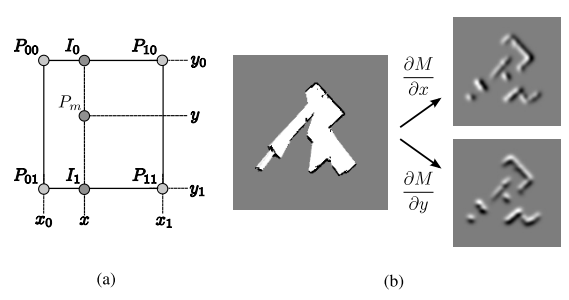
\includegraphics[width=0.7\linewidth]{figs/hectorSLAM_filtering}
%----------------------------------------------------	
	\caption[Hector SLAM aspects of filtering]{The figure illustrates aspects of filtering used to obtain sub-grid cell accuracy. (a) Bi-linear filtering of the occupancy grid map. Point $P_m$ is the point whose value shall be interpolated. (b) Occupancy grid map and spatial derivatives. Taken from \cite{Kohlbrecher2011a}.}
%----------------------------------------------------	
	\label{fig:hectorslamfiltering}
%----------------------------------------------------	
\end{figure}
%....................................................

%

%Equations \ref{eq:gaussnewton} and \ref{eq:hessian} rely on the gradient of the map \(\nabla{M}(P_m)\), where \(P_m\) is some coordinate in the map. Figure \ref{fig:hectorslamfiltering}illustrates the gradient approximation by a bilinear filter of the four closest coordinates(\(P_{00},P_{01}, P_{10},P_{11} \)) representing the midpoints of the surrounding map cells of \(P_m\). The gradient of the map can be approximated as
%\begin{equation}
%\frac{\delta{M}}{\delta{x}}(P_m) \approx (y-y_0)[M(P_{11} - M(P_{01}]+(y_1-y)[M(P_{10}) -M(P_{00})]
%\end{equation},

%\begin{equation}
%\frac{\delta{M}}{\delta{y}}(P_m) \approx (x-x_0)[M(P_{11} - M(P_{10}]+(x_1-x)[M(P_{01}) -M(P_{00}]
%\end{equation},

%where \(x, y \) are coordinates in the map of integer values \(P\). Another assumption is that %\(x_1 - x_0 = y_1 - y_0 = 1\) in the map coordinates.

%....................................................
\begin{figure}[H]
%----------------------------------------------------
	\centering
	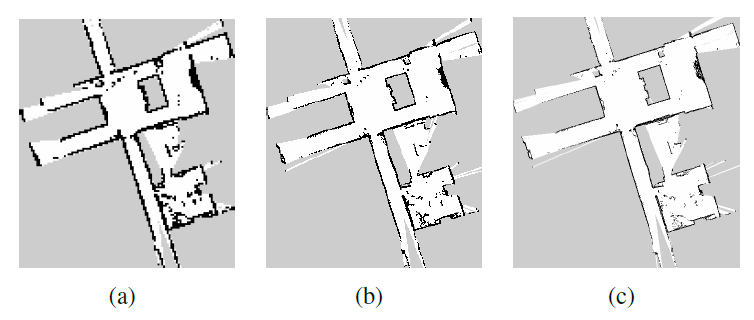
\includegraphics[width=0.7\linewidth]{figs/hectorSLAM_multiresolution}
%----------------------------------------------------	
	\caption[Hector SLAM multi-resolution representation]{Multi-resolution representation of the occupancy grid map: (a): 20 cm occupancy grid cell length (b) 10 cm occupancy grid cell length (c) 5 cm occupancy grid cell length. Where grey cells are unknown, black are occupied cells and white are unoccupied cells.Taken from \cite{Kohlbrecher2011a}.}
	\label{fig:hectorslammultiresolution}
%----------------------------------------------------	
\end{figure}
%....................................................

The scan matching is further optimised to reduce the effect of getting stuck in local minima as the procedure is based on gradient ascent. The optimisation is achieved by using \textit{image pyramids}, where the map is stored at different resolutions. Scan matching is then done at all levels of the image pyramid starting from the coarsest to finest representation. Instead of implementing a computationally costly method such as Gaussian filtering or down-sampling, at the different layers LIDAR scans are written at the scale of each map. The method of writing LIDAR scans to maps, ensuring computational effectiveness and consistency, see Figure \ref{fig:hectorslammultiresolution} \cite{Habbecke2006IterativeM}.

To help the scan matching algorithm, odometry and other position data sources can estimate the scan match. This initial estimation can be done with a Kalman filter or other methods of sensor fusion.

Hector SLAM discussed in this section solves the SLAM problem sufficiently accurately for both ground and water robots \cite{Kohlbrecher2011a}. Hector SLAM has proven to require half the computation time as FastSLAM requires \cite{Eliwa2017}. Furthermore, the approach does not require any explicit loop closing in the considered scenarios, due to  \cite{Kohlbrecher2011a}.  

%----------------------------------------------------
\subsection{Summary}

Even though all four paradigms discussed in previous sections perform in some instances, they have limitations associated with them, influencing the navigation block's performance, shown in Figure \ref{fig:autoover}. The fundamental needed for navigation in robots is an algorithm that covers high-level specifications of humans' tasks into low-level descriptions of how to move. For example, imagine being giving two computer-aided-design(CAD) models: a house and a piano. An algorithm is then expected to move the piano from one room to another without colliding with any obstacles. This problem is referred to as the \textit{Piano Mover's Problem} and defines the classic navigation problem \cite{lavalle_2006}.

Navigation's main objective is to move an object through the environment without collisions; the object and environment's current state needs to be accurately represented. Since the SLAM algorithm feeds the robot's current position and a local map to the navigation block, as shown in Table \ref{table:SLAM}. The quality of these need to be considered when selecting a SLAM algorithm. 

Shown in Table \ref{table:SLAM} are the limitations of the SLAM paradigms discussed in the previous sections. With a focus on data association, computational complexity and the ability to perform SLAM online. Hector-SLAM is selected in this work due to its robustness to loop closure, ability to perform SLAM online, and lack of dependency on odometry data, which is usually less accurate than modern LIDAR scanners. Furthermore, works done by \cite{Eliwa2017} shows that Hector-SLAM has higher accuracy than FastSLAM, even though its computation time is twice fast as FastSLAM. The representation of local maps passed to the navigation block will be discussed in the next section.

%....................................................
\begin{table}[H]
%----------------------------------------------------
\centering
\caption[SLAM method comparison]{A comparison of the reviewed SLAM methods, highlighting their advantages and disadvantages with regards to loop closure events, computational complexity, online capabilities and map size handling.}
    \begin{tabular}{p{6.5em}p{5.5cm} p{5.5cm}} 
%----------------------------------------------------
\toprule[1.5pt] 
%----------------------------------------------------
\multicolumn{1}{l}{\textbf{Method}}     & \multicolumn{1}{c}{\textbf{Advantages}}  & \multicolumn{1}{c}{\textbf{Disadvantages}} \\ 
%----------------------------------------------------
\midrule[0.5pt]
%----------------------------------------------------
  {\em EKF-SLAM }      & 
%....................................................    
        \begin{compactitem}{\small
%----------------------------------------------------    
        \item Works well with unique observations.
        \item Can perform SLAM online.}
%----------------------------------------------------        
    \end{compactitem}   & 
%....................................................   
    \begin{compactitem}{\small
%----------------------------------------------------    
        \item Computational complexity of $\mathcal{O}(M^2)$, where $M$ is the map size. This complexity makes EKF computationally expensive as the map grows to update the covariance matrix as the map grows.
        \item Susceptible to data association errors due to uni-modal pose representation. Hence, loop closure is more frequent.}
%----------------------------------------------------        
    \end{compactitem}\\
%....................................................
%----------------------------------------------------
\hline
%----------------------------------------------------
   {\em  FastSLAM  }     &
%....................................................    
    \begin{compactitem}{\small
%----------------------------------------------------    
        \item Overcomes the loop closure problem, with multi-modal data association.
        \item Copes well with nonlinear and non-Gaussian systems.
        \item Can perform SLAM online.}
%----------------------------------------------------        
    \end{compactitem}   &
%....................................................    
    \begin{compactitem}{\small
%----------------------------------------------------    
        \item Suffers from particle deprivation. Which limits long-term exploration.
        \item Becomes computationally expensive as the map size $M$ grows and the number of particles $Q$ increases, giving a computational complexity of $\mathcal{O}(Q \log M)$.}
%--------Q-, which -------------------------------------------        
    \end{compactitem}\\ 
%----------------------------------------------------
\hline
%----------------------------------------------------
   {\em GraphSLAM   }   & 
%....................................................    
    \begin{compactitem}{\small
%----------------------------------------------------    
        \item Ideal for building large-scale maps.
        \item Overcomes the loop closure problem.}
%----------------------------------------------------        
    \end{compactitem}   & 
%....................................................   
    \begin{compactitem}{\small
%----------------------------------------------------    
        \item Computationally expensive if not optimised. 
        \item Can not perform SLAM online effectively.}
%----------------------------------------------------        
    \end{compactitem}\\ 
%----------------------------------------------------
\hline
%----------------------------------------------------
  {\em   Hector SLAM }    &
%....................................................    
    \begin{compactitem}{\small
%----------------------------------------------------    
        \item Does not require loop closure.
        \item Hector SLAM depends on modern LIDAR scanners rather than odometry data which is less accurate. 
        \item Can perform SLAM online.
        \item Hector SLAM is two times fast computationally compared to FastSLAM \cite{Eliwa2017}.}
%----------------------------------------------------         
    \end{compactitem}   &
%....................................................    
    \begin{compactitem}{\small
%----------------------------------------------------     
       \item Initial guess of the pose may take longer to converge if odometry data are not used to initialise the scan matcher algorithm.} 
%----------------------------------------------------        
    \end{compactitem}\\
%....................................................
\bottomrule[1.5pt] 
%----------------------------------------------------
\end{tabular}
%----------------------------------------------------
\label{table:SLAM}
%----------------------------------------------------
\end{table}
%....................................................

%====================================================
\section{Map representation}
%----------------------------------------------------
The SLAM block discussed in the previous section produces both a local map and current robot pose in the map. The representation of the map depends on how the map is going to be used. For example, in the \textit{Piano Mover's Problem} discussed in the previous section, a piano requires moving from room to room. In this case, our assumptions will be a three-dimensional environment with room labels. In other examples, robots may need all objects in the environment labelled. Therefore, an effective map representation is required to match the scenario. In the case of this thesis, the map representation needs to be compatible with merging maps generated from multiple robots to form a global map of the environment. 

There are various types of map representations, varying from geometrical to logical maps which have been developed to date; the following factors characterise the complexity of mapping problem \cite{Thrun2006}:

%....................................................
\begin{itemize}
%----------------------------------------------------
    \item \textbf{Size}: If the environment size is larger than the relative perceptual range of the robot, mapping becomes more difficult. This makes it more challenging to compute the full posteriors over maps.
%----------------------------------------------------
    \item \textbf{Noise perception and actuation}: Noise on the sensors and actuators of the robot decreases the accuracy, as the errors accumulate.
%----------------------------------------------------
    \item \textbf{Perceptual ambiguity}: If different locations look-alike more frequently, it is more difficult to establish a correspondence between the locations at different time points.
%----------------------------------------------------
    \item \textbf{Loop Closure}: With odometry error, it is easier to correct if the robot travels up and down a corridor. The difficulty comes when a robot re-enters a location from a different path. This same problem was a point of discussion in the previous sections.	
%----------------------------------------------------
\end{itemize}
%....................................................

%----------------------------------------------------
\subsection{Occupancy grid maps}
%----------------------------------------------------
Occupancy grid maps were first introduced in the 1980s and are one of the most common map representations \cite{Siciliano2008b}. In the approach is represented by discrete cells. Where the posterior probability is calculated to determine if a cell is occupied or not, in the case of range sensors, cells will be empty if rays are unobstructed and rays that have an endpoint will be observed as occupied. Occupancy grid maps also account for unknown space, where the area of the map has not been explored as yet. Figure \ref{fig:exampleofoccupancygrid} is an example of an occupancy grid map created using a laser range finder. Black represents occupied cells, white represents empty cells, and grey represents unexplored territory.

%....................................................
\begin{figure}[H]
%----------------------------------------------------
	\centering
	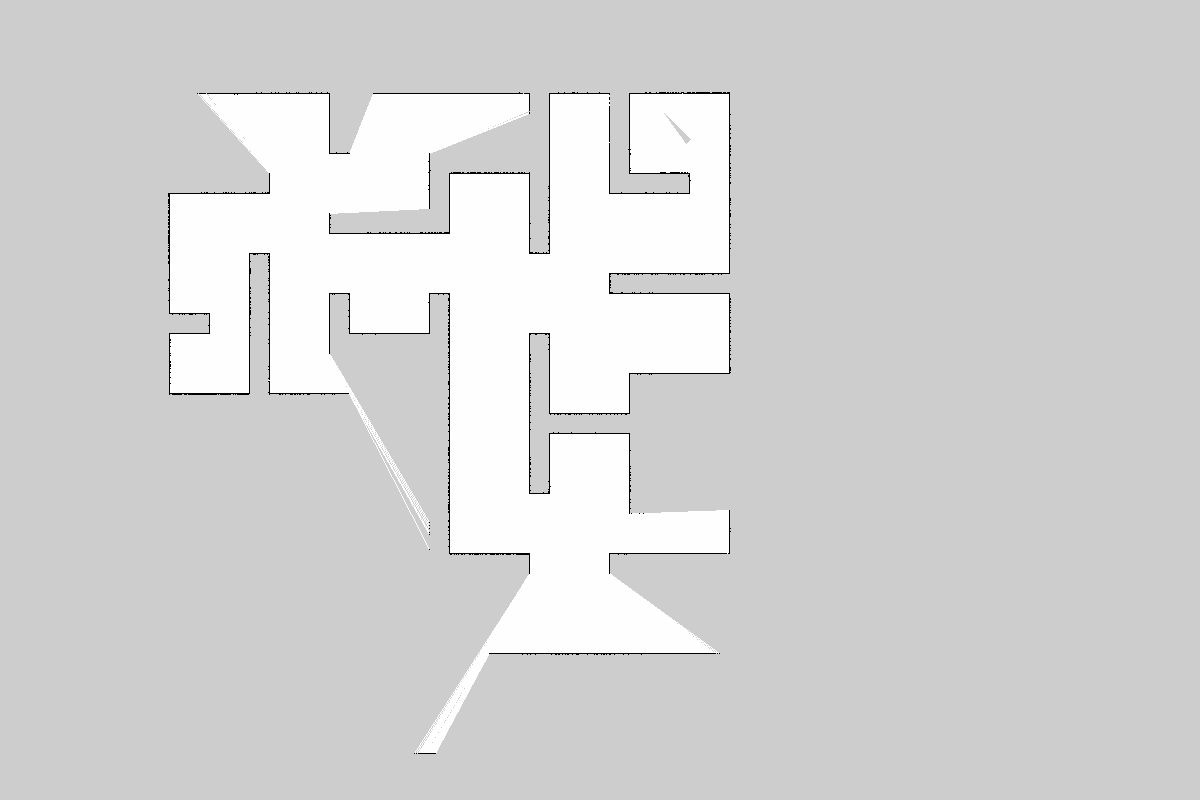
\includegraphics[width=0.7\linewidth]{figs/example_of_occupancy_grid}
%----------------------------------------------------	
	\caption[An example of an occupancy grid map]{An example of an occupancy grid map, which was produced in simulation using Gazebo and ROS (explanation of how the data were acquired is explained in further chapters). Black represents occupied cells, white represents empty cells, and grey represents unexplored territory.}
	\label{fig:exampleofoccupancygrid}
%----------------------------------------------------	
\end{figure}
%....................................................

During an exploration, new sensor observations are used to update the grid cells according to the \textit{Binary Bayes Filter}. The belief of a particular cell \(\mathbf{m}_i\) is given by:

\begin{equation}
%----------------------------------------------------
    bel_{k}(\mathbf{m}_i) = P(\mathbf{m}_i|\mathbf{z}_{1:k},\mathbf{x}_{1:k}),
%----------------------------------------------------
\end{equation}

where ,$\mathbf{m}$, represents the entire map, $\mathbf{m}_i$, is an individual cell in the map, $\mathbf{z}_{1:k}$, is a set of measurements and $\mathbf{x}_{1:k}$ is the pose of the robot at time ,$k$. Therefore the belief for the entire map ,$\mathbf{m}$, is given by:
%....................................................
\begin{equation}
%----------------------------------------------------
    bel_{k}(\mathbf{m}) = \prod_{i}P(\mathbf{m}_i|\mathbf{z}_{1:k},\mathbf{x}_{1:k}).
%----------------------------------------------------    
\end{equation}
%....................................................
A common approach is to represent the belief using \textit{log-odds} \cite{Thrun2001b}:
%....................................................
\begin{equation}
l_{k,i} = \log \frac{P(\mathbf{m}_i|\mathbf{z}_{1:k},\mathbf{x}_{1:k})}{1-P(\mathbf{m}_i|\mathbf{z}_{1:k},\mathbf{x}_{1:k})},
\end{equation}
%....................................................
the \textit{log-odds} representation is used to avoid numerical instabilities for probabilities near zero or one. The probabilities can be recovered using:
%....................................................
\begin{equation}
%----------------------------------------------------
P(\mathbf{m}_i|\mathbf{z}_{1:k},\mathbf{x}_{1:k}) = 1 - \frac{1}{1 + \exp {l_{k,i}}}.
%----------------------------------------------------
\end{equation} 
%....................................................
Finally combining the \textit{log-odds} beliefs can be represented as:
%....................................................
\begin{equation}
%----------------------------------------------------
    l(\mathbf{m}_i|\mathbf{z}_{1:k},\mathbf{x}_{1:k}) = l(\mathbf{m}_i|\mathbf{z}_{1:k-1},\mathbf{x}_{1:k-1}) + l(\mathbf{m}_i|\mathbf{z}_{k},\mathbf{x}_{k}). 
%----------------------------------------------------
\end{equation}
%....................................................

The advantage of these types of maps is that they can handle the dynamic environment, do not rely on predefined features, offer constant-time access to grid cells, and represent unobserved areas \cite{Siciliano2008b, Saeedi}. However, when dealing with dynamic environments, the drawback is that unlearning that a cell is free requires as much observation as the robot received to declare the area occupied \cite{Siciliano2008b}.

These maps also have disadvantages which mainly pertain to high memory requirements (when working in higher dimensions). Therefore, even though 3D maps (called voxels) can be represented using this representation, the implementation will have high memory costs\cite{Saeedi}.

%----------------------------------------------------
\subsection{Feature (as known as landmark) maps}
%----------------------------------------------------
When environments have distinguishable features such as a pillar or tree, for example, landmark-based map representations are typically used. Signatures of the features are usually used to occupy the position of the feature. This representation is more efficient of localisation as the landmark features are initially defined, but feature extraction (data association) is the drawback to this implementation\cite{Siciliano2008b}.
%----------------------------------------------------
\subsection{Topological Maps}
%----------------------------------------------------
Topographical representation was firstly presented in work done by \cite{Kuipers1991} and is one of the more popular mapping techniques. This technique represents the environment in a graph-like structure, focusing on the geometric structure of the environment. In topological mapping, unique, distinguishable places are defined as nodes, and the connections between the nodes are edges where the robot can travel \cite{Siciliano2008b}. 

Topological maps can also be derived from metric maps such as occupancy grids. An example of a Voronoi graph topological map presented in \cite{2005i} produced a topological map from an occupancy grid map. A metric-free topological maps approach is introduced in \cite{Derenick2013}, enabling minimalistic robot localisation.

Note that topological maps are well suited for high-level planning but need intensive map processing, and they are limited in way-point following \cite{Saeedi}.

%----------------------------------------------------
\subsection{Summary}
%----------------------------------------------------
In selecting the appropriate representation for this work, the representations need to be favourable for both map merging and navigation (see Table \ref{table:maprep} for characteristics of the different approaches). Thus, occupancy grid map representation has been selected for their flexibility when representing the environment, and do not require as much computational ability as Feature and Topological maps \cite{Thrun2006}. In the case of map merging, they allow for image registration, and optimisation based approaches \cite{Saeedi}. Occupancy grid maps can also be abstracted to topological maps for navigation \cite{Saeedi}.
%....................................................
\begin{table}[H]
%----------------------------------------------------

\centering
\caption{Map representation characteristics}
\label{table:maprep}
%----------------------------------------------------
\footnotesize
\begin{tabular}{p{4.5em} p{5.5cm} p{4cm} p{4cm}} 
%----------------------------------------------------
\toprule[1.5pt] 
%----------------------------------------------------
\multicolumn{1}{l}{\textbf{Type of Map}} & 
\multicolumn{1}{c}{\textbf{Characteristics}} &
\multicolumn{1}{c}{\textbf{Pros}} &
\multicolumn{1}{c}{\textbf{Cons}}  \\ 
%----------------------------------------------------
\midrule[0.5pt]
%------{\em Occupancy Grid Maps}---------------------	
		{\em Occupancy Grid Maps} &
%....................................................   
		The map is defined as a grid, where each cell is either occupied, free or unknown. &
		
%.................................................... 	
        It is easy to build, probabilistic, suitable for 2D maps, easy to maintain, and suited for low-level planning. & Expensive on fine resolutions and 3D representations, exponential cost of memory with growing size. \\
%....................................................
%----------------------------------------------------
\hline
%----------------------------------------------------
		{\em Feature Maps} & 
%....................................................		
		Maps are represented by landmarks such as trees and shapes. & 
%....................................................
		Very useful for localisation. & Requires computationally expensive data association.\\
%....................................................
%----------------------------------------------------
\hline
%----------------------------------------------------
		{\em Topological Maps} & 
%....................................................
		Abstract spacial information is used to represent the maps. & 
%....................................................
		It is suited for high-level planning. & Is limited to way-point.\\
%....................................................
\bottomrule[1.5pt] 
%----------------------------------------------------		
	\end{tabular}
%----------------------------------------------------	
\end{table}
%....................................................

%====================================================
\section{SLAM extended to Multiple Robots}
\label{sec:SLAMMR}
%----------------------------------------------------
This section will briefly describe multiple-robot systems and multiple-robot SLAM. Generally, multiple robot SLAM algorithms are built on top of single robot SLAM systems; therefore, methods and map representation are based on the approaches mentioned previously. Jung suggests that the following advantages drive research in the field of multiple-robot SLAM \cite{Jung2000}:
%....................................................
\begin{itemize}
%----------------------------------------------------
\item \textbf{Space and time distribution} - Multiple robots can be in many places while performing different tasks simultaneously. This allows robots to, for example, explore a vast area in a shorter period.
%----------------------------------------------------
\item \textbf{Simpler is better} - In the multiple agent case, each robot can be more straightforward rather than have a single agent that is complex. This simplicity not only decreases the cost of each agent but increases reliability and robustness (see Figure \ref{fig:relvscomp}).
%----------------------------------------------------
\item \textbf{Divide and conquer} - Certain problems are best solved when divided into smaller problems and distributed among the robots.
%----------------------------------------------------
\end{itemize}
%....................................................

%....................................................
\begin{figure}[H]
%----------------------------------------------------
    \centering
    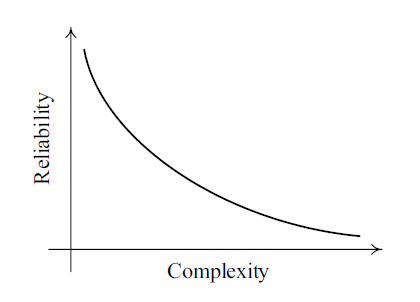
\includegraphics{figs/relability_vs_complexity.png}
 %----------------------------------------------------   
    \caption[Relationship between reliability and complexity]{Relationship between reliability and complexity. The figure suggests that the simpler the system, the more reliable it is. Taken from \cite{Jung2000}.}
    \label{fig:relvscomp}
%----------------------------------------------------    
\end{figure}
%....................................................

However, having a multiple robots system has its associated problems. According to \cite{Saeedi}, these are the potential problems:
%....................................................
\begin{itemize}
%----------------------------------------------------
    \item \textbf{Relative poses} - Maps produced by individual autonomous robots are referred to as local maps, which are produced in the robot's frame of reference. To produce a global map, each robot needs to incorporate maps from all the robots. This can be difficult as it requires transformation matrices to relate the maps to each other. The relative pose also has its associated uncertainty which can be represented as a covariance matrix. This uncertainty can be caused by modelling, sensor noise, and linearisation effects \cite{Thrun2006}. 
%----------------------------------------------------    
    \item \textbf{Updating maps and poses} - After the relative transformation matrix has been found, the local maps need to be fused; thus, the poses also need to be updated. The process needs to consider the robot trajectory and new information added to the local maps. The processes also need to consider the type of map; for example, in feature-based maps, duplicate landmarks may need to be removed \cite{Siegwart2004}.
 %----------------------------------------------------   
    \item \textbf{Line-of-sight observations} - Line-of-sight observation is when robots can see or detect each other. Even though robots might already possess the other robots' pose estimation, line-of-sight can improve the estimates.  In some cases, this can be more reliable than the indirect approaches, but in some cases, robots might not have a sight of each other, especially during a mission such as search and rescue \cite{DeHoog2009}. Furthermore, line-of-sight has been used in loop closure scenarios \cite{Matari2004}.
%----------------------------------------------------    
    \item \textbf{Loop closure} - This happens when a robot revisits a previously visited location but not very recently. As the issue is already complicated enough for single robot missions \cite{Balcilar2016}, extending this to multiple robots, the issue requires information from the robots in the system to be solved \cite{Howard2006a}.
 %----------------------------------------------------   
    \item \textbf{Complexity} - Especially when considering that usually robotic applications are real-time, space and time advantages mentioned above are essential to solving the multi-robot SLAM problem with minimum time and memory requirements. This complexity directly affects the scalability of the multi-robot SLAM operation.
%----------------------------------------------------    
    \item \textbf{Information sharing} - The quality of the information sharing among the robots mainly depends on the medium and environment which they are communicating \cite{Carlone2010a}. For example, underwater robots face different issues to that of aerial robots. Different environments introduce different limitations to bandwidth, data rate and throughput.
%----------------------------------------------------    
    \item \textbf{Homogeneous vs. heterogeneous} - Having a diverse robot team can be a considerable advantage, especially in different terrain environments, this allows for a wholesome model of the environment. For example,  a team may have robots on the ground, in the air and underwater \cite{Siciliano2008b}. The synchronisation between the different robots and sensors, is an essential part of multiple robot systems, firstly on each robot and all the robots. However, this advantage requires processing and integrating different types of robots \cite{Wurm2012}, such as integrating different map representations.
 %----------------------------------------------------   
    \item \textbf{Performance measure} - Measuring the accuracy of multiple robot systems, can be challenging considering the issues mentioned above and the lack of a model of the environment. This process is essential, primarily if the robot relies on SLAM to coordinate and perform tasks. Performance measures can be used to ensure the reliability of multiple-robot SLAM systems.
%----------------------------------------------------    
\end{itemize}
%....................................................

Furthermore, in Multiple Robot SLAM can either be centralised or decentralised \cite{Leung2010}. In a \textbf{centralised system}, there is a predetermined robot in the team or an external agent which handles the computation of tasks. The assumption is that the central agent has a global map of the ``World'', which theoretically means that the central agent can optimally allocate tasks to the robot team. The robots would need to send partial maps continuously to the central agent, and the central agent will be responsible for aligning and merging the maps then the maps would be sent back to the robot team to produce the global map. This requires constant communication between the robot's in the team and the central agent. The central approach can either be implemented wholly (apart from the central agent other, agents have no control or autonomy) or partially (there is still a central agent, but other agents can also take some autonomous local decisions). 

In a \textbf{decentralised system}, more than one robot is tasked with performing computations for tasks. However, it requires each robot to have adequate computational ability to act independently. In the map merging case, the robots may exchange maps with each other then align and merge them internally. The global map built by each robot may vary depending on which robots they have exchanged information.

Centralised systems allow for coherent and comprehensive solutions. However, depending on the size of the team in a centralised system it may become difficult or impractical to store all the information of the environment on one agent \cite{Leung2010}, a communication bottleneck may arise due to the massive communication between the central agent and other agents, high complexity leads to low reliability as per the following Figure \ref{fig:relvscomp}. On the other hand, a decentralised system is tolerant to failure, reliable and robust, scalable, and tasks can be decomposed and run in parallel compared to the centralised approach \cite{Leung2010}.

In this section, the advantages and disadvantages of Multiple Robot SLAM are discussed. In the next section, related work on Multiple Robot SLAM is discussed concerning these advantages and disadvantages.

%====================================================
\section{Related work on Multiple Robot SLAM}
%----------------------------------------------------
In the previous section, three key advantages (space and time distribution; simplicity; and divide and conquer) and eight fundamental problems (relative poses of robots; uncertainty of the relative poses; updating maps and poses; line-of-sight observations; closing loops, complexity communications; team diversity; synchronisation and performance measures) of multiple-robot SLAM were discussed, which are adapted from \cite{Saeedi}. Furthermore, the centralised vs. decentralised multiple-robot SLAM systems are discussed. The following section will explore multiple-robot SLAM solutions.

Several researchers proposed the Multi-Robot SLAM problem, with work dating back to the early 2000s such as \cite{Nettleton2000}. \cite{Nettleton2000} applied the information formulation to the multiple-robot SLAM problem; the work shows that the Extended Information Filter (EIF) is more suitable than EKF multiple-robot SLAM since the information has the additivity attribute. However, the authors noted that data association and communication between robots would need to be further researched.  

Later \cite{Thrun2005} improved on the work done by \cite{Nettleton2000}, by proposing a multiple-robot SLAM with Sparse Extended Information Filers (SEIF). An algorithm that enables robot teams to build joint maps where the relative starting position is unknown and landmarks are ambiguous. The alignment of local maps to generate a global map is achieved by a tree-based algorithm which searches for local landmarks arrangements combined with a hill-climbing method to maximise the overall likelihood. 

Fenwick et al. propose an EKF based multiple-robot SLAM approaches and explore merging sensor and navigation information from multiple robots \cite{Fenwick2003}. The method is based on stochastic estimation and uses a feature-based map representation, where a theoretical convergence theorem is proved for the first time. This approach quantifies gains of using a team of robots, therefore determining the number of robots required in a team to perform tasks.

Another EKF based multiple-robot SLAM technique is proposed by \cite{Rekleitis2001}, where a team of robots (both stationary and dynamic) directly observe each other to reduce the dead reckoning errors. Furthermore, the algorithm is designed to cope with hard-to-sense reflectance properties. 

Later, \cite{4058636} proposed an EKF based multiple-robot SLAM technique, which aimed to solve the with the aid of robots rendezvousing to consolidate the relative position. In the method, robots do not require knowledge of their initial relative poses to merge maps to form a joint map. Furthermore, the method optimises the map merging and not the map overlap. 

In \cite{Andersson2008}, a multiple-robot SLAM method using Square Root Information Smoothing is presented. This method allows a team of robots to built a global without initial information of the robots relative poses, during a line-of-sight observation. In contrast to EKF approaches, the smoothing is better equipped to deal with the nonlinear process and measurement models. The method joins the maps from different robots and recovers each robot's complete trajectory in the map merging process.

In 2001 Thrun \cite{thrun2001a} proposed a multiple-robot SLAM solution based on a particle filter, where the fast maximum likelihood map grows with a Monte Carlo localiser that uses a particle representation. This yields an online algorithm that can cope with significant odometric errors, typically found when dealing with loop closures. However, the method has the following limitations: firstly, it cannot handle nested cycles in the map, secondly does not deal well with lower quality range sensors such as sonar sensors, and thirdly robots need to know their initial relative poses to each other.  

Later in 2006, the work was extended by \cite{Howard2006a}, where a multiple-robot SLAM using Rao–Blackwellised particle filter was proposed. The robots use line-of-sight to estimate relative position, using cameras and unique markers mounted on them. At the first meeting point, a Rao–Blackwellised particle filter (RBPF) is applied to the data in reverse time sequence to fuse all the data from the starting point, to determine relative position. Furthermore, the maps and poses are updated in real-time, and the decentralised nature of the system increases reliability, robustness and the scalability of the approach. However, it cannot be applied if the robots cannot see each other, and are unable to determine their relative positions. 

Carlone \cite{Carlone2010a} similarly explores multiple-robot SLAM using the RBPF extending on \cite{Howard2006a}'s work relative initial position of the robots are unknown. In this work, the main focus is information sharing among the robots, with limited communication between them. The information shared when the robots are in-range includes all the odometry and corresponding laser range-finder data. Line-of-sight observation is used then to compute the relative pose with an incorporated uncertainty. 

In \cite{VidalCalleja2011}, a heterogeneous multiple-robot SLAM algorithm using sub-map matching is developed on a team of robots comprised of one ground robot and a helicopter. A global graph maintains the relative relationships between the local sub-maps. Monocular cameras are used as the primary exteroceptive sensors in this work. 3D points are estimated using an inverse-depth parametrisation, 3D line segments are estimated by adding endpoints to extend anchored Pl\"ucker coordinates (a coordinate system that assigns six homogeneous coordinates to each line in projective 3D-space\cite{ZHAO2014113}).

In \cite{Quraishi2016}, robustness to connectivity loss for multiple-robot SLAM method is proposed. In the framework, no central authority is required while the robot team contributes to the global map. However, this method requires systematic coordination among the robots in order to add to the global map. Hence, if a robot leaves the system unannounced, it can potentially make the map inconsistent.

Work done by \cite{Balcilar2016} proposes a Hector mapping architecture for multi-robot. In their work (which they implemented in ROS), each robot shares its observations and poses a central note. The central node computes the global map, using the poses (including the initial poses) and observations from the robot team. Furthermore, parallelising optimisation steps and sequentially registering laser scans to the jointly built map are implemented to enable real-time running. Table \ref{table:multisolution} states the algorithms' main features in this section.
%....................................................
\begin{table}[H]
%----------------------------------------------------
    \centering
    \caption{Solutions to Multiple Robot SLAM problems }
%----------------------------------------------------
\begin{tabular}{p{5cm}p{5.5cm}} 
%----------------------------------------------------
    \toprule[1.5pt]
%----------------------------------------------------   
\multicolumn{1}{l}\textbf{Problem} & 
\multicolumn{1}{c}\textbf{Solutions}\\ 
%----------------------------------------------------    
    \midrule[0.5pt]
 %----------------------------------------------------   
    {\em Relative poses}        & 
    \cite{Thrun2005}, \cite{4058636}, \cite{Rekleitis2001}, \cite{Carlone2010a}, \cite{VidalCalleja2011}, \cite{Quraishi2016}\\ 
%----------------------------------------------------     
   % \hline 
   & \\  
%----------------------------------------------------   
   {\em Updating maps and poses}      & 
   \cite{Thrun2005},\cite{Fenwick2003},\cite{Howard2006a}, \cite{VidalCalleja2011}, \cite{Andersson2008}, \cite{Quraishi2016}\\
 %---------------------------------------------------- 
    %\hline
     & \\  
 %----------------------------------------------------   
    {\em Line-of-Sight observations}  & 
    \cite{Rekleitis2001},\cite{4058636},\cite{Howard2006a}, \cite{Andersson2008}\\
 %----------------------------------------------------   
    %\hline
     & \\  
 %----------------------------------------------------   
     {\em Loop closure}               & 
    \cite{Rekleitis2001}, \cite{thrun2001a}\\ 
 %----------------------------------------------------   
  %  \hline
   & \\  
 %----------------------------------------------------   
     {\em Complexity}               & 
    \cite{Howard2006a}, \cite{Balcilar2016}, \cite{Andersson2008}\\
 %----------------------------------------------------
   %  \hline
    & \\  
%----------------------------------------------------     
     {\em Information sharing}         & 
    \cite{Carlone2010a}, \cite{Quraishi2016}\\
 %----------------------------------------------------
   % \hline
    & \\  
%----------------------------------------------------   
    {\em Homogeneous vs. Heterogeneous} & 
    \cite{VidalCalleja2011} \\
 %----------------------------------------------------   
   % \hline
    & \\  
 %----------------------------------------------------   
    {\em Performance measures}         & 
   \cite{Fenwick2003}\\
%----------------------------------------------------    
    \bottomrule[1.5pt]
%----------------------------------------------------   
\end{tabular}
%----------------------------------------------------
\label{table:multisolution}
%----------------------------------------------------
\end{table}
%....................................................

%====================================================
\section{Summary}
%----------------------------------------------------
In this chapter, an overview of SLAM is explored, including SLAM formulation, single robot SLAM solutions, map representation, and multiple-robot SLAM extension. The multiple-robot SLAM literature, problems such as relative poses, updating maps and pose and homogeneous vs. heterogeneous are discussed in Section\ref{sec:SLAMMR}, along with some solutions that tackle the problems. The work done in this chapter, also prompts the use of Hector SLAM as the SLAM algorithm each robot will be equipped; occupancy grid maps as the map representation; and a distributed architecture where robots communicate when they discover each other in the network. In the next chapter, merging maps from single independent robots are discussed, along with details on how maps are acquired, how robots share maps, and how they are aligned and merged.
%****************************************************
% END
%****************************************************
